\documentclass[a4paper,11pt]{article}
\usepackage[utf8]{inputenc}
\usepackage{amsmath}
\usepackage{amsfonts}
\usepackage{amssymb}
\usepackage{graphicx}

\numberwithin{equation}{section}
\renewcommand\thesubsection{\alph{subsection}}
\newcommand{\bvp}[1]{\mathbf{#1}'}
\newcommand{\bv}[1]{\mathbf{#1}}
\newcommand{\pp}[1]{#1'}


%opening
\title{Computational properties of neural microcolumns arising from temporal dynamics}
\author{Vince Baker, advisor: Dr. Luis Cruz Cruz\\ Drexel University Department of Physics}

\begin{document}

\maketitle

\section{Introduction} 
The human brain hosts advanced cognitive processes that remain only partially understood.
Computational neuroscience seeks to understand brain functions through modeling at several levels of physical fidelity.
``Biologically inspired'' computation models are used in machine learning to solve a variety of problems that are intractable with conventional approaches.
Computational biophysics provides insight into the lowest levels of neural functions while nonlinear dynamics provides tools for understanding some aspects of cognition.
This research will explore the computational properties of neural networks through a novel combination of biophysics, nonlinear dynamics and machine learning.
\\ \\
\section{Review of neural network dynamics}
First part: review of basic neural dynamics.
Discuss Hodgkins-Huxley experiment, differential equations leading to dynamic behavior.
Include graphic showing various neural models, highlight Izhikevich (MATLAB) and HH (NEURON) models for this work.\\
Second part discusses cortex organization into columns and microcolumns.
Includes previous results from the group on structure and synchronization.
Introduce SPIKE metric for synchronization.\\
\\ \\
\section{Review of neural column computational properties in a liquid state machine}
This section reviews the liquid state machine architecture.
Focus on fading memory concept and the separation and approximation properties.\\
\\ \\
\section{Initial results: Temporal dynamics in a small neural column}
Introduce simple column structure.
Review distance-based connection probability.
\\
\begin{figure}
 \caption{Column structure}
 \centering
   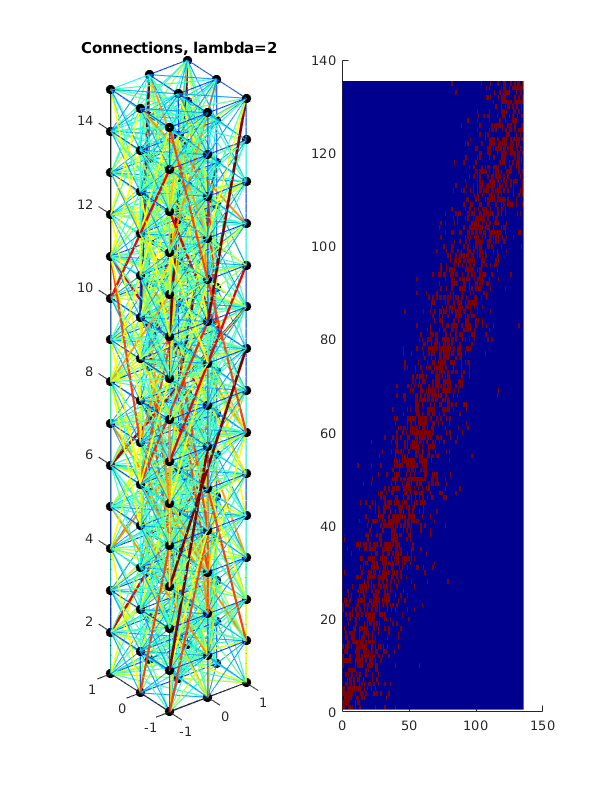
\includegraphics[width=200px]{fig/lambda2}
\end{figure}
\\
Present Izhikevich model enhanced with length-dependent synaptic delays.
Compare approach with Maas Liquid State Machine, we are adding more realistic delay dynamics.
Figure below show two columns with identical neurons with identical connectivity, top has random delays while bottom has distance-dependent delays.
Demonstrates importance of delay dynamics.
\\
\begin{figure}
 \caption{Column structure}
 \centering
   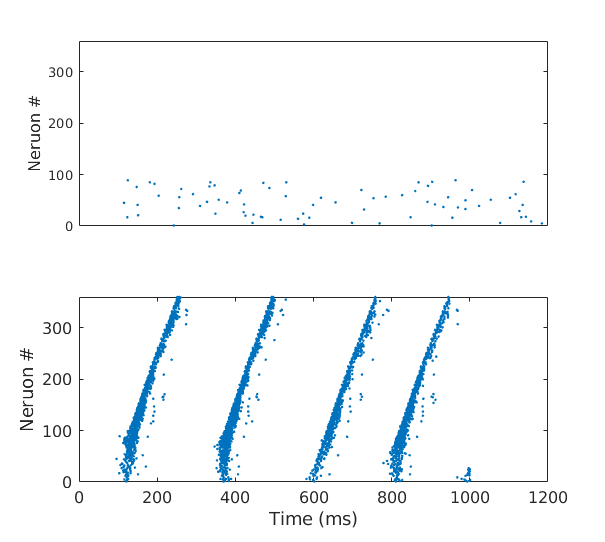
\includegraphics[width=\textwidth]{fig/DelayCompare_RandInput}
\end{figure}
\\

Discuss action potential velocity (typically 1-100 m/s), seems too fast for delay dynamics to matter in real networks.
Effective velocity can depend on column structure (figure below). 
Might be an important feature of microcolumn structure, to be explored in thesis.
\\
\begin{figure}
 \caption{Effective propagation velocity}
 \centering
   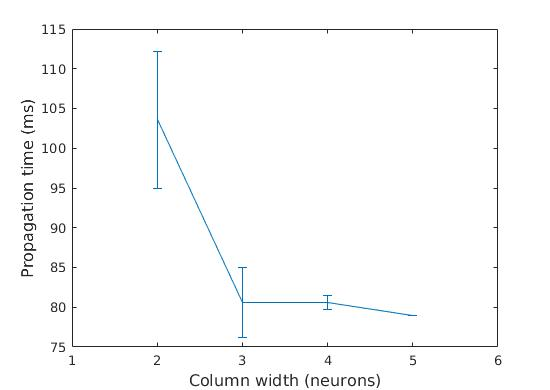
\includegraphics[width=\textwidth]{fig/propagation_time}
\end{figure}
Neural dynamics near a bifurcation can result in a delayed firing (Izhikevich).
Could be another mechanism for slower effective velocity.
\\ \\
Introduce SPIKE metric and input/output distances-fading memory with association.
Compare to Maas Liquid State Machine measures of similarity.
\\
\section{Suggestions for further research}
Further investigation into mechanisms for lower effective velocity: spatial organization, neuron dynamics.\\


\end{document}
